% !TEX root = calculus_iii_midterm.tex
\settasks{
    label=\arabic*.,
    label-align=left,
    label-width=0.8em
}

\setlength\headheight{0pt}  % header height
\setlength\footskip{48pt}    % space before base of footer
\addtolength\textheight{40pt}
\renewcommand{\headrulewidth}{0pt} % width of header line
\fancyhead[L,R]{}
\fancyfoot[C]{\fbox{\bf หน้าที่ \thepage}}

\renewcommand{\qmark}[1]{\textit{(#1\ คะแนน)}}
\newcommand{\ansbox}{\ensuremath{\boxed{\hspace*{7em}\vphantom{\dfrac12}}} {}}
\newcommand{\ansboxs}{\ensuremath{\boxed{\hspace*{4em}\vphantom{\frac12}}} {}}
\newcommand{\ansboxl}{\ensuremath{\boxed{\hspace*{10em}\vphantom{\frac12}}} {}}
\newcommand{\ansboxL}{\ensuremath{\boxed{\hspace*{12em}\vphantom{\frac12}}} {}}
\newcommand{\ansboxq}{\ensuremath{\boxed{\hspace*{2em}\vphantom{\frac12}}} {}}
\newcommand{\ansboxi}[1]{\ensuremath{\boxed{\hspace*{#1}\vphantom{\frac12}}} {}}
\newcommand{\polarcoordinatecircle}{
    \medskip
    \begin{center}
        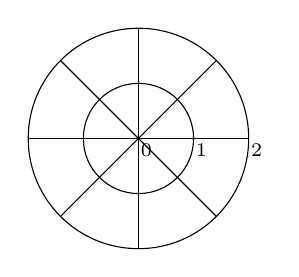
\begin{tikzpicture}[font=\scriptsize,scale=0.7]
            \draw (0,0) circle(1);
            \draw (0,0) circle(2);
            \foreach \i in {0,45,...,315} {
                    \draw (0,0) -- (\i:2);
                }
            \foreach \i in {0,1,2} {
                    \node[below,shift={(0.1,0.05)}] at (\i,0) {$\i$};
                }
        \end{tikzpicture}
        \hspace*{1cm}
    \end{center}
}
\usetikzlibrary{patterns}
\newcommand{\polarcoordinatetheta}{
    \begin{center}
        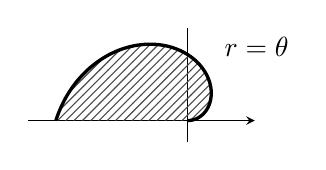
\begin{tikzpicture}
            \begin{axis}[
                    scale=0.42,
                    axis lines=middle,
                    y axis line style={-},
                    xmin=-3.8, xmax=1.6,
                    ymin=-0.5, ymax=2.2,
                    ticks=none,
                    axis equal image
                ]
                \addplot[
                    domain=0:pi,
                    samples=100,
                    pattern=north east lines,  % Hatching pattern
                    pattern color=black!70,
                    draw=none
                ]
                (
                {x*cos(deg(x))},
                {x*sin(deg(x))}
                )
                \closedcycle;
                \addplot[
                    domain=0:pi,
                    samples=100,
                    very thick,
                    black
                ]
                (
                {x*cos(deg(x))},
                {x*sin(deg(x))}
                );
            \end{axis}
            \node at (2.9, 1.2) {$r = \theta$};
        \end{tikzpicture}
        \hspace*{2.7cm}
    \end{center}
}
\newcommand{\polarcoordinatesintwotheta}{
    \begin{center}
        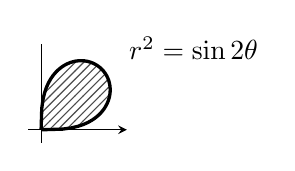
\begin{tikzpicture}
            \begin{axis}[
                    scale=0.22,
                    axis lines=middle,
                    y axis line style={-},
                    x=1cm, y=1cm,
                    xmin=-0.15, xmax=1,
                    ymin=-0.15, ymax=1,
                    ticks=none,
                    axis equal image
                ]
                \addplot[
                    domain=0:pi,
                    samples=100,
                    pattern=north east lines,  % Hatching pattern
                    pattern color=black!70,
                    draw=none
                ]
                (
                {sqrt(sin(deg(2*x))) * cos(deg(x))},
                {sqrt(sin(deg(2*x))) * sin(deg(x))}
                )
                \closedcycle;
                \addplot[
                    domain=0:pi,
                    samples=101,
                    very thick,
                    black
                ]
                (
                {sqrt(sin(deg(2*x))) * cos(deg(x))},
                {sqrt(sin(deg(2*x))) * sin(deg(x))}
                );
            \end{axis}
            \node at (2.1, 1.2) {$r^2 = \sin 2 \theta$};
        \end{tikzpicture}
        \hspace*{2.7cm}
    \end{center}
}